\chapter{Splotowe sieci neuronowe}
Splotowe sieci neuronowe są wielowarstwowymi sieciami jednokierunkowymi. Charakteryzuje je~możliwość
wykrywania wzorców występujących w~różnych fragmentach przetwarzanego obrazu (np. rozpoznawanie oka
w~dowolnym fragmencie obrazka). Zasada ich~działania była inspirowana neurobiologią, a~mianowicie analizowano
sposób przetwarzania informacji przez~ośrodek wzrokowy kota.

\section{Filtry splotowe}
Splot dyskrentny jako pojęcie matematyczne jest zdefiniowany w~następujący sposób:
$$ f\ast g[n]\defeq \sum\limits_{m=-\infty}^{\infty}f[m]g[n-m] = \sum\limits_{m=-\infty}^{\infty}f[n-m]g[m]$$
gdzie $f$ i $g$ to~ciągi splatane, a~zapis $f[n]$ to~zapis oznaczający $n$-ty wyraz ciągu $f$.

W~cyfrowym przetwarzaniu obrazów filtry splotowe znajdują bardzo szerokie zastosowanie, gdyż w~zależności
od~dobranej maski filtra, osiągane są różne rezultaty.

\subsection{Przykładowe filtry splotowe}
\subsubsection{Filtr Gaussa}
By~lepiej zrozumieć działanie filtrów splotowych warto posłużyć się~przykładami. Jednym z~najczęściej stosowanych
mechanizmów tego typu jest filtr Gaussa, którego zadaniem jest wygładzenie (inaczej: rozmazanie) obrazu.
Maska tego filtru została przedstawiona na~rysunku \ref{rys:maska-gauss}.
\begin{figure}[H]
	\centering
	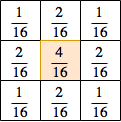
\includegraphics[width=0.25\linewidth]{img/gauss-conv-kernel.png}
	\caption{Maska filtru Gaussa}
	\label{rys:maska-gauss}
\end{figure}

Dla~obrazu źródłowego (patrz rys.~\ref{rys:img-src-gauss}), aby~otrzymać obraz przekształcony
(rys.~\ref{rys:output-gauss}) należy policzyć średnią ważoną dla~otoczenia każdego przekształcanego piksela, a~więc:
\begin{enumerate}
    \item Przemnożyć wartość każdego piksela z~odpowiadającą mu wartością maski.
    \item Dodać wszystkie iloczyny do~siebie.
    \item Znormalizować uzyskaną wartość poprzez podzielenie jej przez~sumę wag tworzących maskę (krok wykonywany tylko
    przy~wykorzystaniu niektórych filtrów).
\end{enumerate}

Tak~uzyskana wartość to~w~przekształconym obrazie nowa wartość piksela. Operacja splotu jest zwykle wykonywana
dla~każdego piksela oryginalnego obrazu.

\begin{figure}[H]
	\centering
	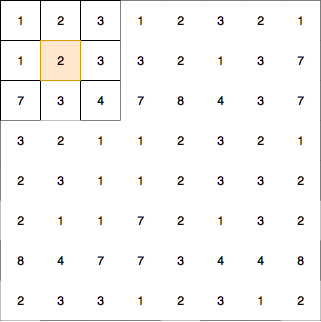
\includegraphics[width=0.5\linewidth]{img/gauss-conv-src-img.png}
	\caption{Przykładowy obraz, który może zostać przekształcony przy~użyciu filtru Gaussa. Poszczególne wartości
	w~komórkach odpowiadają wartościom pikseli w~obrazie niekolorowym (odcienie szarości)}
	\label{rys:img-src-gauss}
\end{figure}

\begin{figure}[H]
	\centering
	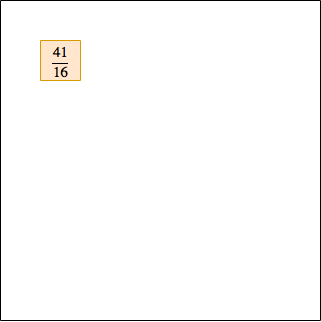
\includegraphics[width=0.5\linewidth]{img/gauss-conv-output.png}
	\caption{Obraz zawierający piksel przekształcony przy~użyciu filtru Gaussa}
	\label{rys:output-gauss}
\end{figure}

Efekt działania filtru Gaussa na~prawdziwym obrazie przedstawiono na~rysunku \ref{rys:gauss-conv-example}.
\begin{figure}[H]
	\centering
	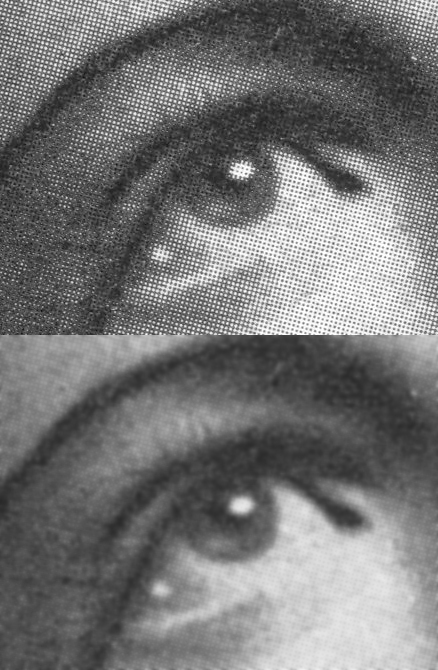
\includegraphics[width=0.4\linewidth]{img/gauss-conv-real-example.jpg}
	\caption{Efekt działania filtru Gaussa na~prawdziwym obrazie. Na~górze: obraz oryginalny, na~dole: obraz
	przekształcony}
	\label{rys:gauss-conv-example}
\end{figure}

Jak~można zaobserwować, w~filtrze Gaussa na~nową wartość piksela mają częściowo wpływ piksele sąsiednie
i~przede~wszystkim stara wartość piksela.

\subsubsection{Filtr Laplace'a}
Zadaniem tego filtru jest wyostrzanie obrazu. Efekt ten jest osiągany poprzez usunięcie wpływu sąsiednich pikseli
na~wartość każdego przekształcanego piksela. Jest to~poniekąd filtr o~działaniu odwrotnym do~filtru Gaussa. Jądro splotu
dla~omawianego mechanizmu przedstawiono na~rysunku \ref{rys:maska-laplace}.

\begin{figure}[H]
	\centering
	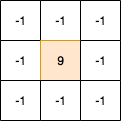
\includegraphics[width=0.25\linewidth]{img/laplace-conv-kernel.png}
	\caption{Maska filtru Laplace'a}
	\label{rys:maska-laplace}
\end{figure}

Działanie filtru Laplace'a zaprezentowano na~rysunku \ref{rys:laplace-conv-example.jpg}.

\begin{figure}[H]
	\centering
	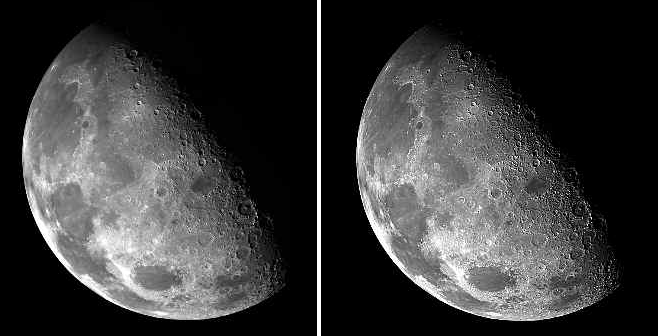
\includegraphics[width=\linewidth]{img/laplace-conv-example.png}
	\caption{Efekt działania filtru Laplace'a na~prawdziwym obrazie. Po~lewej: obraz oryginalny, po~prawej: obraz
	przekształcony}
	\label{rys:laplace-conv-example}
\end{figure}

Maski dla~zaprezentowanych filtrów (tj.~dla~filtru Gaussa i~filtru Laplace'a) są~z~góry ustalone i~nie~ulegają zmianie
w~czasie działania algorytmu.

Splotowa sieć neuronowa zamiast wykorzystywać z~góry określone maski, ,,uczy się ich'',
a~więc stara się~tak dobrać ich~wagi, aby~jak~najlepiej rozpoznawać wyznaczone obiekty na~obrazach. Poszczególnym
wartościom w~masce filtra odpowiadają wagi splotowej sieci neuronowej.

\subsection{Dopełnienie (\textit{ang.~padding})}
Przy~stosowaniu filtrów splotowych pojawia się problem: jaką wartość powinny otrzymać piksele obrazka
znajdujące się na~jego krawędzi. Jest on~rozwiązywany poprzez rozszerzanie obrazka o~dodatkowe piksele
na~jego krawędziach. Można tego dokonać m.in. poprzez:
\begin{itemize}
  \item dopełnienie obrazka czarnymi pikselami (\textit{ang.~zero-padding}),
  \item dopełnienie obrazka odbiciami lustrzanymi pikseli przy krawędziach.
\end{itemize}

\section{Inferencja} \label{sec:inferencja}
W~trakcie działania sieci na~obrazie dokonywanie jest filtrowanie splotowe (przy wykorzystaniu różnych
filtrów). Po~takim filtrowaniu otrzymywane jest $n\cdot m$ obrazów, nazywanych mapami cech
(\textit{ang.~feature maps}), gdzie n~-~liczba początkowych obrazów (tzw.~kanałów wejściowych), m~-~liczba
użytych filtrów.

Po~dokonaniu filtrowania splotowego obrazy są skalowane na~mniejsze (tzw.~faza pooling/subsampling) i~znów
stosowane są~filtry splotowe. Oba kroki (filtrowanie i~skalowanie) są~powtarzane wielokrotnie
(liczbwa powtórzeń zależy od~architektury sieci), aż~do~osiągnięcia odpowiednio wysokopoziomowych cech (patrz
rys.~\ref{rys:convnet-illustration}). Liczba warstw oraz liczba filtrów splotowych wykorzystanych w~każdej z~nich jest
ustalana podczas fazy projektowania sieci.

\begin{figure}[H]
	\centering
	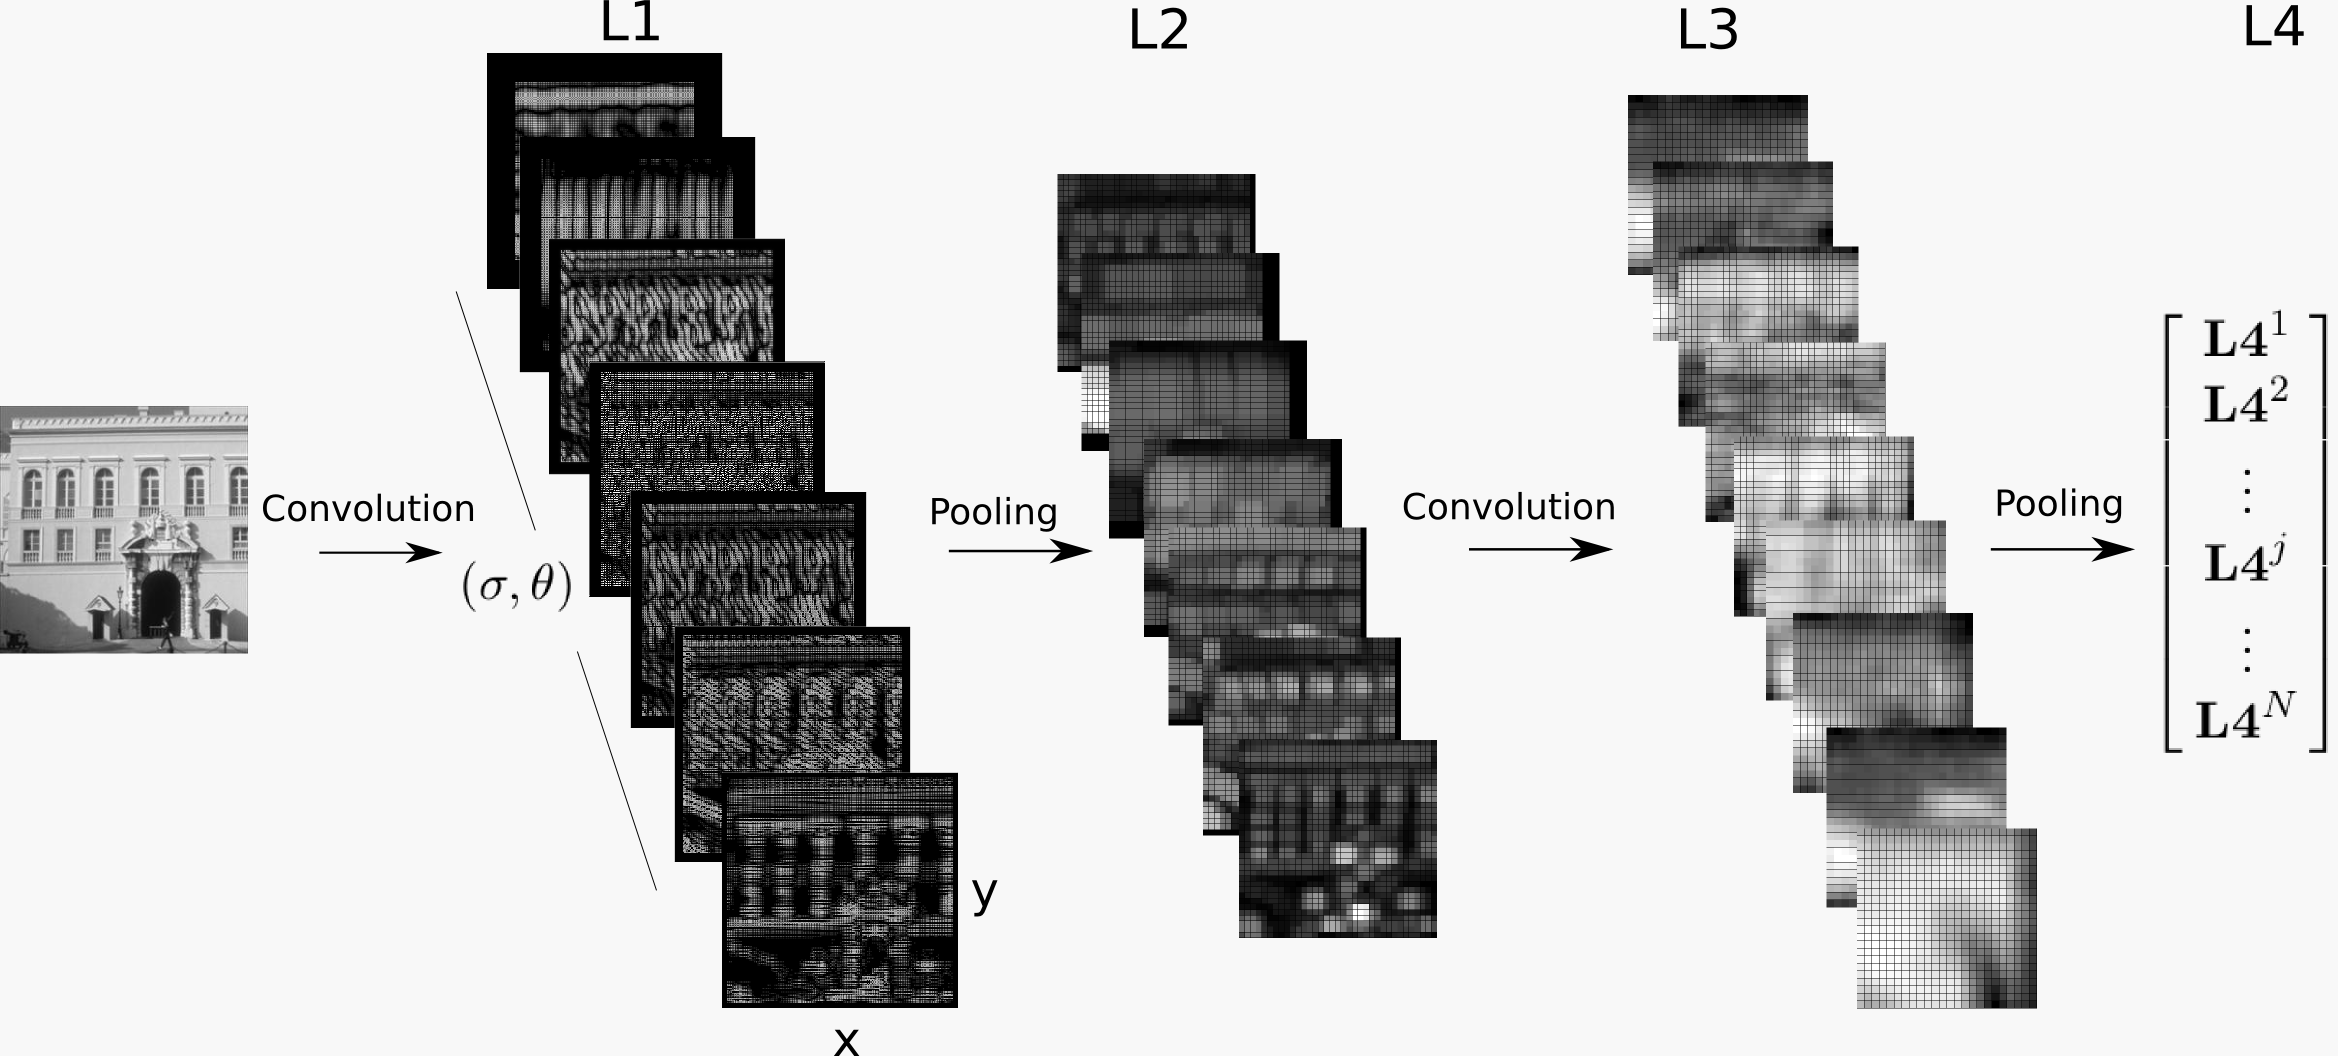
\includegraphics[width=\linewidth]{img/convnet.png}
	\caption{Sieć splotowa, w~której naprzemiennie występują warstwy splotowe i~warstwy skalujące.
	Źródło:~\cite{convnet-illustration}.}
	\label{rys:convnet-illustration}
\end{figure}

Ostatnią warstwą sieci (zazwyczaj otrzymującą dużo bardzo małych obrazów) jest warstwa zawierająca neurony
sigmoidalne. Każdy neuron warstwy wyjściowej jest połączony ze~wszystkimi wartościami otrzymanymi na~wyjściu
poprzedniej warstwy.

\subsection{Skalowanie}
Po zastosowaniu n różnych filtrów splotowych w~danej warstwie na~m~różnych mapach cech, powstaje $n\cdot m$
kolejnych map cech. Stąd ilość przetwarzanych danych szybko rośnie wraz z~dokładaniem kolejnych warstw
w~sieci. Aby temu przeciwdziałać stosuje się skalowanie obrazów pomiędzy warstwami dokonującymi splotu.
Najczęściej obraz skalowany jest poprzez:
\begin{enumerate}
  \item podzielenie obrazka na~nienachodzące na~siebie kwadratowe obszary,
  \item wybranie z~każdego obszaru piksela o~największej wartości (\textit{ang.~max-pooling}).
\end{enumerate}

Alternatywnie, w~drugim kroku algorytmu można wybrać medianę wartości pikseli\\
(\textit{ang.~mean-pooling}) lub~wartość średnią (\textit{ang.~average-pooling}).

\subsection{Normalizacja}
W~sieciach splotowych często stosowanym zabiegiem, mającym na~celu zapewnienie lepszej jakości klasyfikacji jak również
szybszego uczenia, jest normalizacja danych. Operacja normalizacji może być interpretowana jako kolejna warstwa
umieszczana w~sieci na~tej~samej zasadzie, co~warstwa dokonująca splotu czy~warstwa skalująca.

\subsubsection{Lokalna normalizacja odpowiedzi} \label{sssec:normalizacja_odpowiedzi}
\textbf{Lokalna normalizacja odpowiedzi} (\textit{ang.~local response normalization}, \cite{HOG}) polega na~zapewnieniu,
że~wartości pikseli o~podobnych współrzędnych, jednak należące do~różnych map cech, należą do~rozkładu normalnego
o~odchyleniu standardowym równym 1 i~średniej równej 0. Normalizacja polega więc na~odjęciu od~wszystkich pikseli
średniej (liczonej wzdłuż różnych map cech) i~podzieleniu ich przez~odchylenie standardowe (również liczone wzdłuż
rożnych map cech).

Choć wartości odchylenia standardowego i~średniej liczone są z~uwzględnieniem wszystkich map cech, to~nie~muszą
się ograniczać do~jednego piksela. Zamiast tego mogą dotyczyć pewnego jego sąsiedztwa. Metoda ta~odpowiada
mechanizmowi obecnemu w~ośrodkach wzrokowych ssaków, u~których również dla pewnego sąsiedztwa punktu widzianego
obrazu kontrast jest normalizowany. Przykładem tego efektu jest sytuacja, w~której obiekt w~zależności od~tego,
w~jakim otoczeniu się~znajduje, wydaje się~mieć inny kolor \ref{img:chess-illusion}.

\begin{figure}[H]
	\centering
	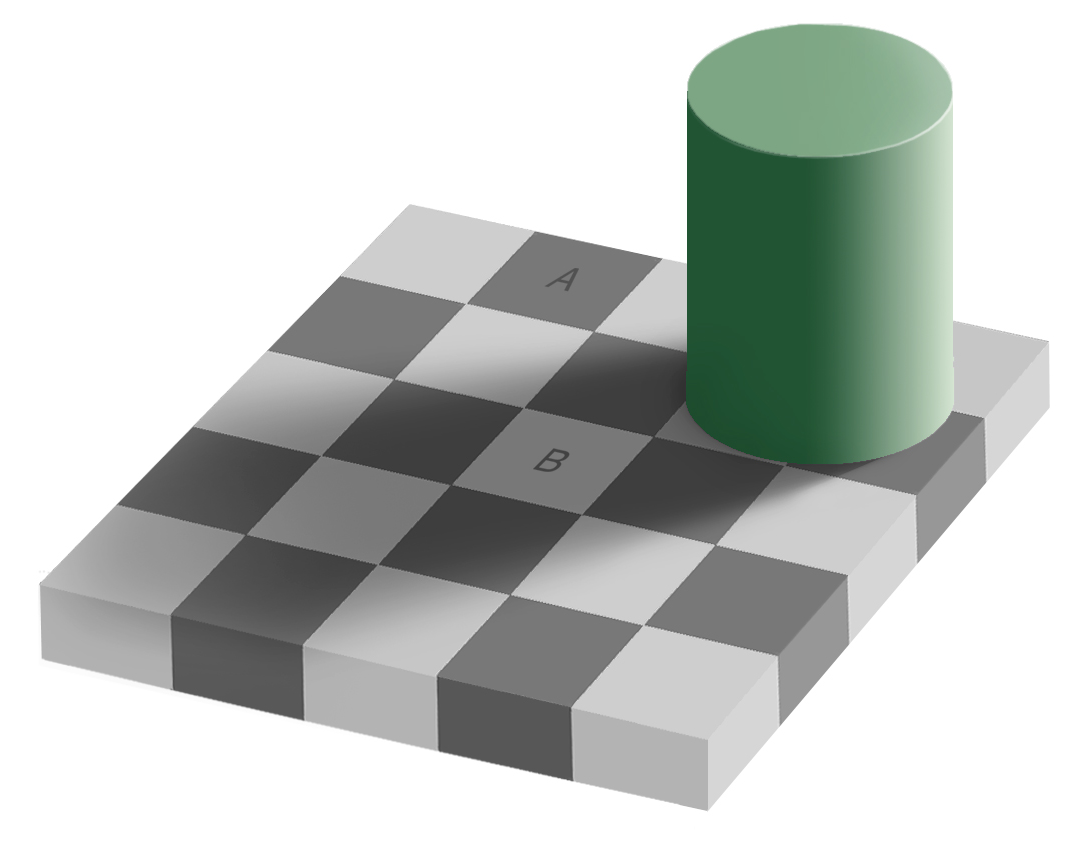
\includegraphics[width=0.8\linewidth]{img/chess-illusion.png}
	\caption{Pola A i B mają ten sam kolor}
	\label{img:chess-illusion}
\end{figure}

\subsubsection{Normalizacja wsadowa}
Jedną z~często stosowanych obecnie metod normalizacji jest tzw.~normalizacja wsadowa (\textit{ang.~batch normalization}).
Jest stosunkowo nową metodą, opublikowaną w~2015 roku (\cite{batch-norm}). Stosuje się~ją jako
dodatkową warstwę umieszczaną za~każdą z~warstw w~pełni połączonych. Warstwa BatchNorm dokonuje normalizacji danych
w~ramach całego wsadu danych (tzw.~batch). Odejmuje~ona od~każdej wartości wejściowej średnią (liczoną dla~przykładów
w~obrębie całego wsadu, dla~każdego z~wejść z~osobna), a~następnie dzieli uzyskane wartości przez~odchylenie standardowe
(liczone analogicznie jak~średnia).
\begin{equation*}
 \widehat{x} = \frac{x - E[x]}{\sqrt{Var(x)}}
\end{equation*}

Tak~znormalizowane dane są~następnie poddawane przekształceniu liniowemu:
\begin{equation*}
y = \gamma\widehat{x} + \beta
\end{equation*}
$\gamma$ oraz $\beta$ są~parametrami, których wartość ustalana jest w~procesie uczenia. Warto zwrócić uwagę, że~jeśli
$\beta=E[x]$ i $\gamma=\sqrt{Var(x)}$ warstwa BatchNorm będzie dokonywała przekształcenia identycznościowego.

Dla~każdej z~operacji wykonywanych przez~tę~warstwę normalizującą można policzyć gradient funkcji kosztu względem
parametrów. Dzięki temu sieć z~warstwami BatchNorm może być uczona metodami gradientowymi, podobnie jak~większość
standardowych sieci.

\subsection{Regularyzacja sieci}
W~przypadku rozpoznawania danych, w~których występować może wiele różnych wzorców, konieczne jest umieszczenie w~sieci
neuronowej dużej liczby neuronów. Jednakże może to~przynieść nieporządany efekt, przy~którym sieć zbytnio dopasuje
się~do~danych (tzw.~overfitting). Sposobem na~ograniczanie tego zjawiska jest \textbf{regularyzacja} sieci.

\subsubsection{Regularyzacja L2} \label{sssec:reg_L2}
Jest~to~prawdopodobnie naczęściej używana forma regularyzacji. By~ją~zastosować, do~funkcji kosztu sieci dodawany
jest człon $\frac{1}{2}\lambda w^2$, a~gradient tego członu to~$\lambda w$. W~efekcie przy~aktualizacji wag wszystkie
z~nich są zmniejszane w~liniowy sposób:
\begin{equation*}
W := W*(1 -\lambda)
\end{equation*}
$\lambda$~to~tzw.~współczynnik regularyzacji, który im~jest większy, tym~bardziej sieć dąży do~tego,
by~mieć równe wartości wszystkich wag (\cite{L2-regularization}).

\subsubsection{Dropout}
Jest to~niezwykle efektywna, a~zarazem prosta technika pozwalająca na~zapobieganie zbytniemu dopasowaniu sieci
do~danych przy~jednoczesnym zapobieganiu \textbf{koadaptacji} neuronów, czyli~sytuacji, w~której różne neurony
przyjmują podobne wagi, przez co~nie~są od~siebie niezależne. Dropout polega na~losowym usuwaniu neuronów z~sieci
podczas procesu uczenia. Dzięki temu w~każdej iteracji uczony jest jedynie pewien podzbiór sieci (\cite{dropout}).

\begin{figure}[H]
	\centering
	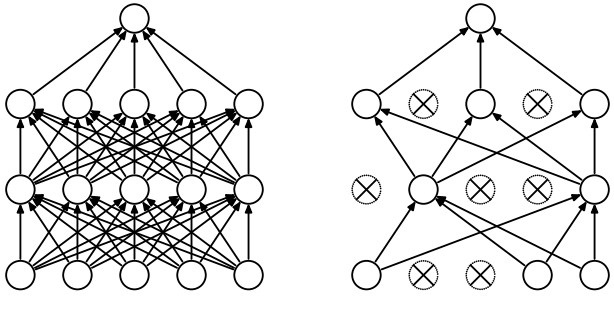
\includegraphics[width=\linewidth]{img/dropout.jpeg}
	\caption{Dropout. Po~lewej: pełna sieć. Po~prawej: sieć po~dokonaniu operacji usuwania losowych neuronów.
	         Źródło: \cite{dropout}}
\end{figure}

\section{Uczenie metodą wstecznej propagacji}
Typową metodą uczenia sieci jest wsteczna propagacja błędów. W~tym celu należy obliczyć gradient funkcji
straty względem wag sieci (wartości masek filtrów splotowych) dla~warstw:
\begin{itemize}
  \item wyjściowych,
  \item skalujących,
  \item splotowych.
\end{itemize}
Obliczanie gradientu funkcji straty dla~warstw zawierających neurony sigmoidalne zostało omówione
w~sekcji (\ref{ssec:backpropagation}), stąd wyjaśnienia wymaga jedynie obliczanie gradientów dla~warstw skalujących i~splotowych.

\subsection{Obliczanie gradientu dla~warstw skalujących}
Znając gradient funkcji straty $\nabla_{y_{ijk}}l$ z~warstwy kolejnej, można w~prosty sposób policzyć gradient
w~stosunku do~wejścia warstwy dla~której jest on liczony. W~przypadku, gdy~warstwa wykorzystywała algorytm
\textit{max-pooling}, gradient względem wejść warstwy przyjme wartość:
\begin{itemize}
  \item $\nabla_{x_ijk}l = \nabla_{y_{ijk}}l$, dla~pikseli, które miały maksymalną wartość w~obszarze, 
  \item $\nabla_{x_ijk}l = 0$, dla~pozostałych pikseli.
\end{itemize}

\subsection{Obliczanie gradientu dla~warstw splotowych}
Przy~wstecznej propagacji błędów z~warstwy kolejnej otrzymujemy gradient błędu względem wyjścia
aktualnej warstwy $\nabla_{y_j}l$. Do~aktualizacji wag sieci konieczne jest policzenie gradientu funkcji
straty wzlgędem wag tej warstwy.
$$ \frac{\partial E}{\partial w_{ab}} 
= \sum\limits_{i=0}^{N-m}\sum\limits_{j=0}^{N-m}\frac{\partial E}{\partial x_{ij}^l}\frac{\partial
x_{ij}^l}{\partial w_{ab}}
= \sum\limits_{i=0}^{N-m}\sum\limits_{j=0}^{N-m}\frac{\partial E}{\partial x_{ij}^l}y^{l-1}_{(i+a)(j+b)}$$
gdzie:
\begin{itemize}
  \item $N\times N$ - rozmiar mapy cech,
  \item $m\times m$ - rozmiar filtra,
  \item $x_{ij}^l$ - wartość wejścia neuronu o~wsp. (i,j) w~warstwie l,
  \item $w_{ab}$ - wartość w~masce filtra znajdująca się~na~pozycji (a,b).
\end{itemize}

Następnie należy policzyć tzw.~delty ($\frac{\partial E}{\partial x_{ij}^l}$):
$$\frac{\partial E}{\partial x_{ij}^l} = \frac{\partial E}{\partial y_{ij}^l}\frac{\partial y_{ij}^l}{\partial
x_{ij}^l} =
\frac{\partial E}{\partial y_{ij}^l}\frac{\partial}{\partial x_{ij}^l}(\sigma(x_{ij}^l))
= \frac{\partial E}{\partial y_{ij}^l}\sigma'(x_{ij}^l)
$$

Na~koniec należy policzyć gradient funkcji błędu względem wyjść warstwy poprzedniej (po~to, by~przekazać
go~do~poprzedniej warstwy):
$$ \frac{\partial E}{\partial y_{ij}^{l-1}} =
\sum\limits_{a=0}^{m-1}\sum\limits_{b=0}^{m-1} \frac{\partial E}{\partial x^l_{(i-a)(j-b)}}
\frac{\partial x^l_{(i-a)(j-b)}}{\partial y_{ij}^{l-1}} =
\sum\limits_{a=0}^{m-1}\sum\limits_{b=0}^{m-1} \frac{\partial E}{\partial x^l_{(i-a)(j-b)}}w_{ab}$$

Należy zwrócić uwagę na~dwie rzeczy: po~piersze na~to, że~podczas obliczania gradientów również wykonywany
jest splot jednak na~obrazku o~,,odwróconych'' wierszach i~kolumnach. Dodatkowo, by~móc dokonywać splotu
na~krawędziach map cech, należy zastosować dopełnienie zerami (\textit{ang.~zero-padding}).

\subsection{Uczenie wstępne}
W~celu lepszego zainicjowania wag sieci należy przeprowadzić uczenie wstępne. W~tym~etapie sieć zamiast uczyć
się rozpoznawania obiektów, ma~za~zadanie nauczyć się~charakteru danych wejściowych (ma~zauważać
charakterystyczne cechy, podobieństwa obiektów it.p.). Do~uczenia wstępnego wykorzystuje się~mechanizmy
uczenia nienadzorowanego, takie jak:
\begin{itemize}
  \item autoenkoder,
  \item RBM (Restricted Boltzmann Machine).
\end{itemize}

Uczenie wstępne przebiega w~następujący sposób:
\begin{enumerate}
  \item wyodrębnienie losowych fragmentów obrazka (tzw.~łatki),
  \item uczenie mechanizmu uczenia nienadzorowanego (np.~RBM),
  \item zainicjowanie wag uczonej warstwy wagami z~tego~mechanizmu,
  \item policzenie map cech dla~łatek,
  \item wykonanie kroków 1-3 dla~uzyskanych map~cech (uczenie wstępne kolejnej warstwy).
\end{enumerate}
